\documentclass[12pt,a4paper]{article}
\usepackage{amsmath}
\usepackage{amsfonts}
\usepackage{amssymb}
\usepackage{graphicx}
\usepackage{secdot}
\usepackage[left=2cm,right=2cm,top=2cm,bottom=2cm]{geometry}

\author{Shibayan Biswas, AE21B109,\\ Department of Aerospace Engineering,\\ IIT Madras\\[3ex] Instructor:\\ \large Professor Dr. Vadlamani Nagabhushana Rao}

\title{Experiment- 2}

\date{November 16, 2022}

\begin{document}

\maketitle
\hline
\section{Aim:}
To construct an approximate Brayton cycle for a micro gas turbine engine on a T-S plot and also to observe the effect of nozzle exit area and afterburner on thrust.
\section{Introduction:}
The first gas turbine that implemented the Brayton Cycle (not knowingly however, because it was created before the Brayton Cycle was even established) was John Barber’s gas turbine patented in 1791. The idea of the machine was to compress atmospheric air in one chamber and fuel in another chamber and both chambers would be connected to a combustion vessel. Once the air has mixed with the fuel and reacted, the energy from the combustion would be used to spin a turbine to do useful work. However, because back in the late 18th century there was lack
of technological advances and such, the gas turbine did not have enough energy to pressurize the gases and do useful work at the same time therefore it was not used. George Brayton was an engineer that designed the first continuous ignition combustion engine which was a two-stroke engine that was sold under the name ”Brayton’s Ready Motors.” The design employed the thermodynamic processes that is now considered ”The Brayton Cycle,” but is also coined The Joule Cycle. The gas turbine was patented in 1872. The design was a engine connected to a reservoir of pressurized atmospheric air and gas which would only turn on if a valve was turned. This would release the pressurized gas to a combustion vessel, which would turn pistons to create mechanical work and re-compress the gas in the reservoir.
\subsection{Brayton Cycle:}
The Brayton Cycle is a thermodynamic cycle that describes how gas turbines operate. The idea
behind the Brayton Cycle is to extract energy from flowing air and fuel to generate usable work which can be used to power many vehicles by giving them thrust. The most basic steps in extracting energy is compression of flowing air, combustion, and then expansion of that air to create work and also power the compression at the same time. The usefulness of the Brayton Cycle is tremendous due to the fact it is the backbone in driving many vehicles such as jets, helicopters, and even submarines.
\subsection{Ideal Brayton Cycle:}
A quick qualitative look at how the Brayton Cycle works it by reviewing how a jet engine works. A gas turbine from a jet’s wing sucks in atmospheric air from the back of its engine and is compressed in the combustion chamber. In the combustion chamber, fuel is mixed with the compressed atmospheric air, where it is ignited and left to exit in the expansion chamber. The energy that comes out of the back of the gas turbine is work used to power the compression step as well as give thrust to the jet.\\
\\The Brayton Cycle can then be described quantitatively in the gas turbine engine of a jet by two diagrams- the Temperature v/s Entropy plot and the Pressure v/s Volume plot as shown below:
\begin{figure}[!ht]
	\begin{center}
		\framebox{
			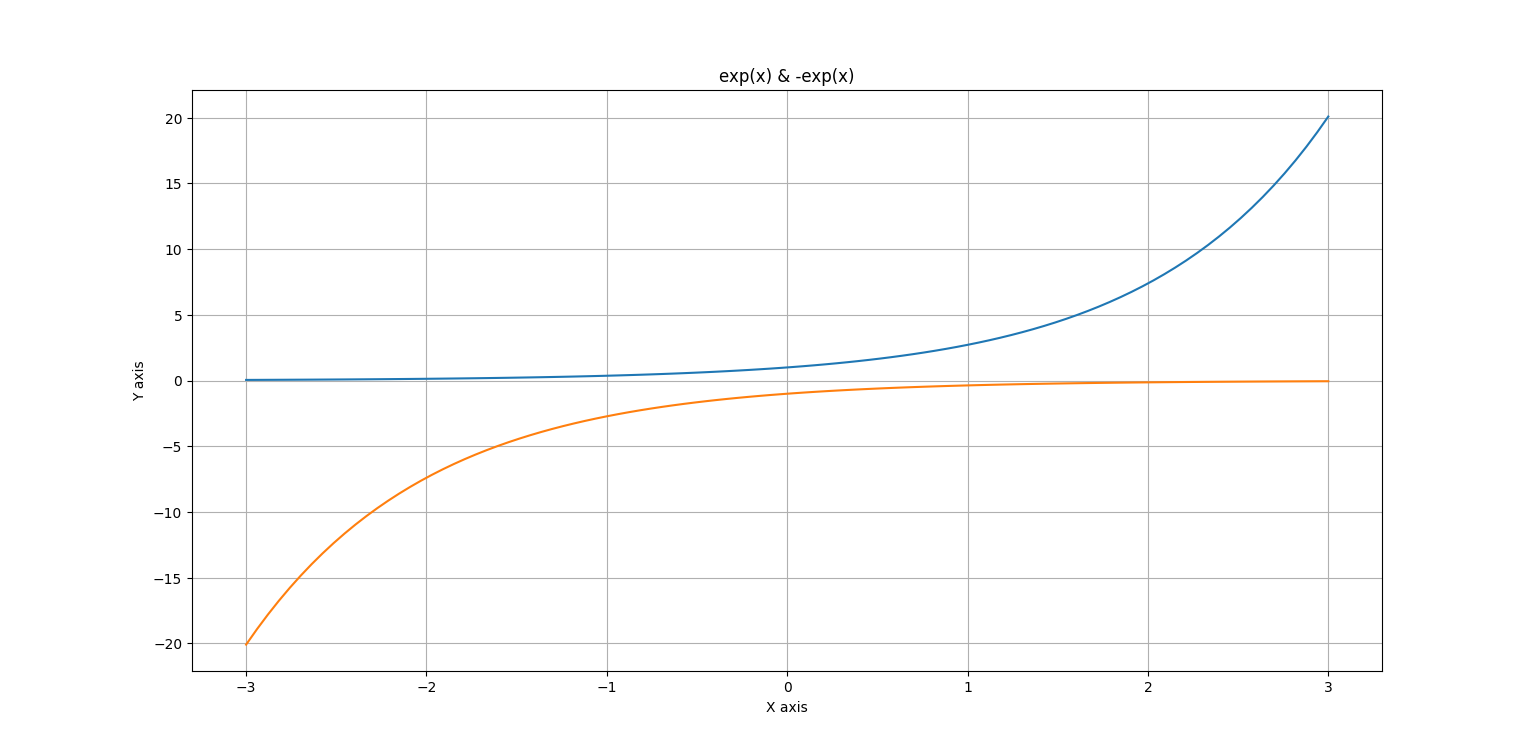
\includegraphics[scale=0.59]{Figure_1.png}
		}
	\end{center}
	\caption{Temperature v/s Entropy plot for Ideal Brayton Cycle}
\end{figure}
\begin{figure}[!ht]
	\begin{center}
		\framebox{
			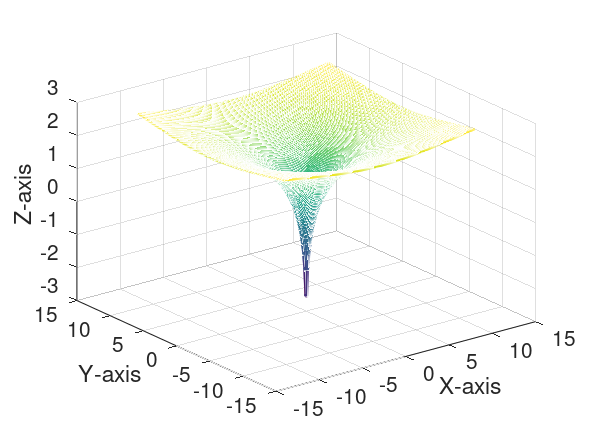
\includegraphics[scale=0.59]{Figure_2.png}
		}
	\end{center}
	\caption{Pressure v/s Volume plot for Ideal Brayton Cycle}
\end{figure}
\section{Theory:}
The ideal processes shown in the above diagrams are used to study and understand the Brayton Cycle better. However, some corrections are needed when applied to real world problems. The first problem is the fact that in the compression process, it is believed to be isentropic. This is wrong, because the high speed flow of the ambient air increases the entropy (higher energy molecules) and thus is not an isentropic process.\\
\\It is actually an adiabatic process because no heat exchange occurs in the gas and only mechanical work is done for compression. This also relates back to the expansion process where the gas expands in the expansion chamber but has yet to leave into the atmosphere. Ideally it is isentropic, but the expansion of gas does increase entropy, therefore it is actually an adiabatic process because again, there is not heat exchange (only mechanical work done by expansion). The non-ideal processes of the Brayton Cycle points out a problem; that the work used to raise
entropy is thus a leak in the amount of work that could have been used for useful mechanical energy. A set of equations is then used to calculate the efficiency of the Brayton Cycle at certain pressures and temperatures.\\
\\A simple gas turbine power plant is shown below. Air is first compressed adiabatically in process a $\textendash$ b, it then enters the combustion chamber where fuel is injected and burned essentially at constant pressure in process b $\textendash$ c, and then the products of combustion expand in the turbine to the ambient pressure in process c $\textendash$ d and are thrown out to the surroundings. The cycle is an open cycle. These type of open cycles are used in aircrafts, automotives and industrial gas turbines.\\
\begin{figure}[!ht]
	\begin{center}
		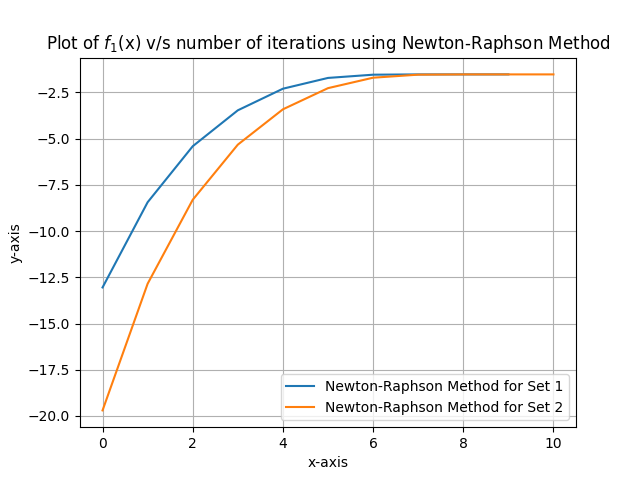
\includegraphics[scale=0.8]{Figure_3.png}
	\end{center}
	\caption{Gas Turbine Plant}
\end{figure}\\
In this cycle air is first compressed reversibly and adiabatically, heat is added to it reversibly at constant pressure, air expands in the turbine reversibly and adiabatically, and heat is then rejected from the air reversibly at constant pressure to bring it to the initial state. The Brayton cycle, therefore, consists of: Two reversible isobars and two reversible adiabats.
\clearpage
\begin{figure}[!ht]
	\begin{center}
		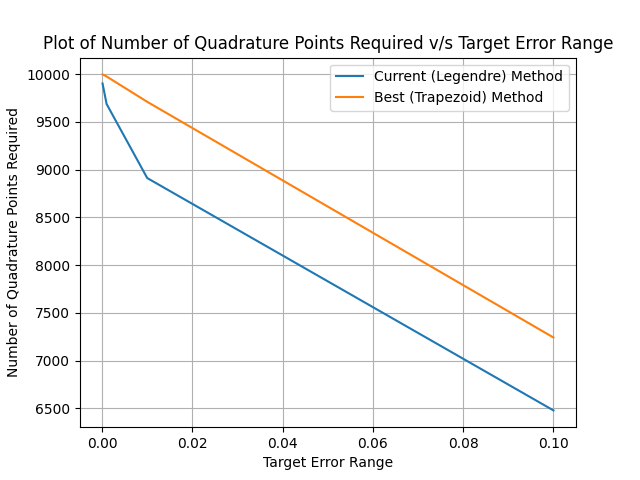
\includegraphics[scale=0.65]{Figure_4.png}
	\end{center}
	\caption{Temperature v/s Entropy plot for Real Brayton Cycle}
\end{figure}
\subsection{Turbo-Jet Engine and Micro-Gas Turbine:}
The micro-gas-turbine (GT RS 100 from TecQuipment, UK) is a self-contained, fully instrumented, educational single shaft gas turbine with afterburner. Powered by kerosene, the experimental abilities of this apparatus enable comprehensive practical investigations into the principles, and performance of single-shaft gas turbines with/without afterburner. It is a steel frame that holds a gas generator, combustion chamber, oil and fuel tanks, pumps, ancillaries and guards.\\
\begin{figure}[!ht]
	\begin{center}
		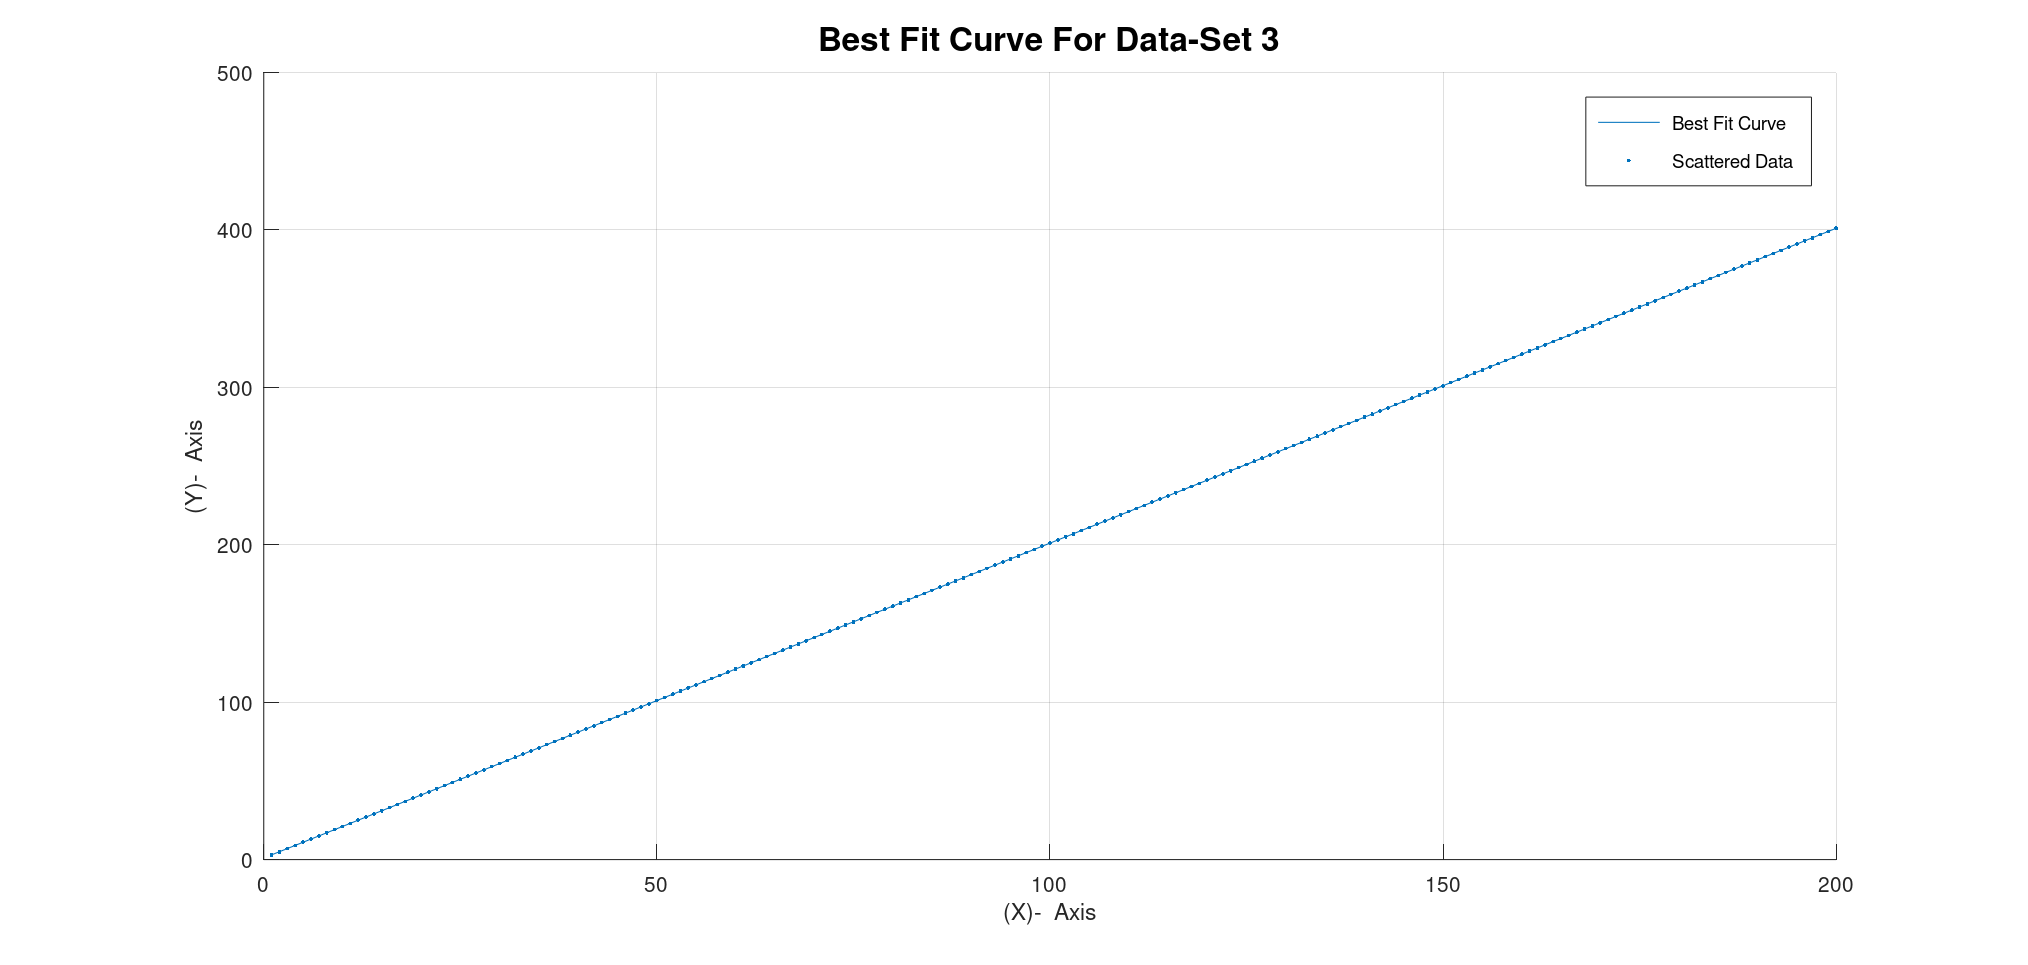
\includegraphics[scale=0.65]{Figure_5.png}
	\end{center}
	\caption{Turbo-Jet Trainer with Afterburner}
\end{figure}
\clearpage
\noindent
\\Above these is an instrumentation and control panel with schematic diagram. The clearly labelled front panel with mimic diagram includes the instrument displays, controls and warning lights. Air passes into an air box, into a radial compressor, then into the combustion chamber.\\
\\A pump transfers fuel from the fuel tank to spray through a special nozzle into the combustion chamber. A high-energy spark ignites the air and fuel mixture, which flows to radial flow turbine, then to the reheat section. This increases the temperature and velocity of the gas. It then
passes through a variable area propelling nozzle. A fuel flow control valve on the instrumentation and control panel allows regulation of the speed.\\
\\Digital indicators show shaft speed, pressures, temperatures and fuel flow. Analogue indicators show fuel level, fuel pressure, oil temperature, oil pressure and hours run. A separate control adjusts the fuel flow to the afterburner section. The Control Panel shows a mimic diagram of the main parts of the equipment, including the Air Box, the compressor, the Combustion Chamber, the turbine, the reheat section and the nozzle. It also has the main controls and displays of pressure, turbine speed, thrust, fuel mass flow, temperatures and nozzle area. The displays allow the user to calculate all the important readings from the turbine and reheat section.\\
\begin{figure}[!ht]
	\begin{center}
		
\includegraphics[scale=1.5]{Figure_6.jpg}
	\end{center}
	\caption{Turbo-Jet Engine}
\end{figure}\\
The operation of a jet engine is represented by the Brayton cycle, a thermodynamic cycle that underlies all gas turbine engines. The Brayton cycle illustrates the thermodynamic processes occurring in an engine, describing how heat and energy are managed by the engine to generate
work, which in the case of a jet engine is propulsive thrust. Throughout the Brayton cycle, through each station of the jet engine, the conditions of the working fluid (air and combustion gases) change.\\
\clearpage
\noindent
Afterburners are added to turbojets to raise the exhaust temperature. This raises the velocity and most usefully, increases the thrust. In practice, afterburners can double the thrust of a turbojet, but will also double the fuel flow. Afterburners rely on the fact that unlike an internal combustion engine, only a very small proportion of the oxygen in the air passing
through the engine is actually burnt. There is sufficient oxygen left in the jet exhaust to be able to sustain a second flame.\\
\begin{figure}[!ht]
	\begin{center}
		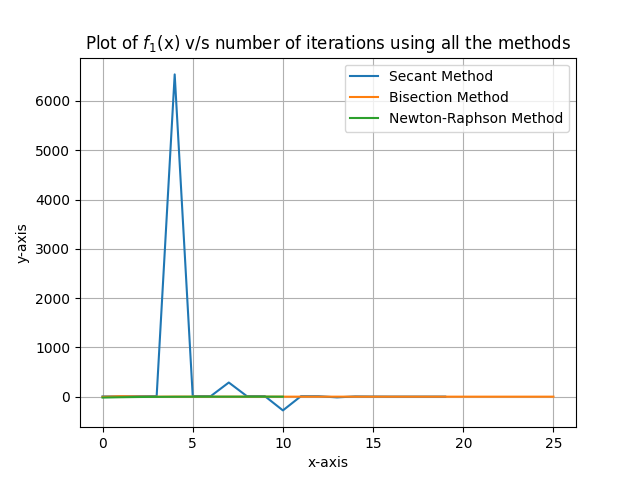
\includegraphics[scale=0.3]{Figure_7.png}
	\end{center}
	\caption{Afterburner Section of Turbo-Jet Engine}
\end{figure}\\
The nozzle has a rectangular cross-section with variable upper and lower sections. These variable sections allow the user to adjust the area of the nozzle. A linear sensor measures the position of the nozzle eyelids.
\clearpage
\subsection{Temperature v/s Entropy Relations for T-S Plots:}
The turbojet engine is characterised and studied by analyzing its Temperature (T) v/s Entropy (S) diagram which shows the variation of Temperature (T) with the Entropy (S) of the system. The working of the turbojet engine comprises of following steps (Please refer to Figure 1):
\begin{itemize}
\item Process 0 $\textendash$ 3 : Isentropic Compression (Compressor)
\item Process 3 $\textendash$ 4 : Constant Pressure Heat Addition (Burner)
\item Process 4 $\textendash$ 5 : Isentropic Expansion (Turbine)
\item Process 5 $\textendash$ 8 : Isentropic Compression (Nozzle)
\end{itemize}
The general governing equation is:
\begin{equation}
    \text{$\Delta s_{AB}$} = \text{$C_p ln$}(\frac{T_B}{T_A}) - \text{$R ln$}(\frac{P_B}{P_A})
\end{equation}
Governing equation for isentropic process:
\begin{equation}
    \text{$C_p ln$}(\frac{T_2}{T_1}) = \text{$R ln$}(\frac{P_2}{P_1})
\end{equation}
Governing equation for isobaric process:
\begin{equation}
   \text{$\Delta s_{23}$} = \text{$C_p ln$}(\frac{T_3}{T_2})
\end{equation}
Firstly there is isentropic compression of the fluid that takes place in the compressor. After that the fluid undergoes isobaric heat addition in the combustion chamber. This is followed by isentropic expansion of the fluid in the turbine. Here, the work done by the fluid on the turbine is transmitted to the compressor by a shaft. We next have the isobaric heat addition to the fluid by the afterburner. This is followed by isentropic expansion in the nozzle. Finally, for the closed cycle considered here, there occurs an isobaric heat rejection bringing the fluid back to the initial state.
\section{Result:}
This particular section contains the results and plots that we have obtained after performing the experiment followed by doing the necessary calculations to derive quantities required for the plots :
\subsection{Case- 1:}
For afterburner off, 100 \% nozzle area, the real readings are as follows:
\begin{itemize}
\item Diffuser: $P_1$ = 1.023 bar, $T_1$ = 300 K.
\item Compressor: $P_2$ = 1.875 bar, $T_2$ = 372 K.
\item Turbine: $P_3$ = 1.695 bar, $T_3$ = 797 K.
\item Afterburner: $P_5$ = 1.01 bar, $T_5$ = 709 K.
\item Nozzle: $P_4$ = 0.935 bar, $T_4$ = 727 K.
\clearpage
\end{itemize}
\begin{figure}[!ht]
	\begin{center}
	   \framebox{
			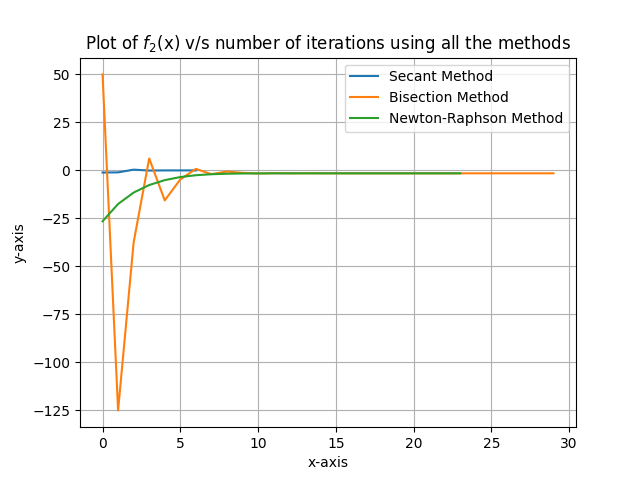
\includegraphics[scale=0.2]{Figure_8.png}
		}
	\end{center}
	\caption{Temperature (T) v/s Entropy (S) diagram for afterburner off, 100 \% nozzle area}
\end{figure}
\subsection{Case- 2:}
For afterburner on, 100 \% nozzle area, the real readings are as follows:
\begin{itemize}
\item Diffuser: $P_1$ = 1.023 bar, $T_1$ = 300 K.
\item Compressor: $P_2$ = 1.865 bar, $T_2$ = 372 K.
\item Turbine: $P_3$ = 1.685 bar, $T_3$ = 805 K.
\item Afterburner: $P_5$ = 1.008 bar, $T_5$ = 1016 K.
\item Nozzle: $P_4$ = 0.935 bar, $T_4$ = 737 K.
\end{itemize}
\begin{figure}[!ht]
	\begin{center}
	   \framebox{
			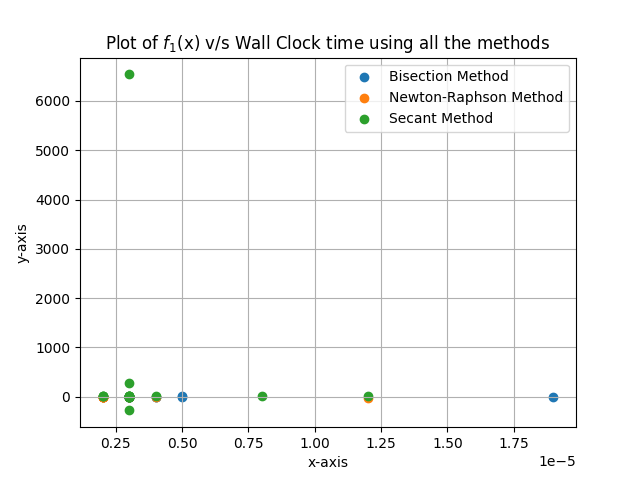
\includegraphics[scale=0.2]{Figure_9.png}
		}
	\end{center}
	\caption{Temperature (T) v/s Entropy (S) diagram for afterburner on, 100 \% nozzle area}
\end{figure}
\subsection{Case- 3:}
For afterburner off, 65 \% nozzle area, the real readings are as follows:
\begin{itemize}
\item Diffuser: $P_1$ = 1.023 bar, $T_1$ = 300 K.
\item Compressor: $P_2$ = 1.865 bar, $T_2$ = 374 K.
\item Turbine: $P_3$ = 1.695 bar, $T_3$ = 817 K.
\item Afterburner: $P_5$ = 1.014 bar, $T_5$ = 738 K.
\item Nozzle: $P_4$ = 0.935 bar, $T_4$ = 746 K.
\end{itemize}
\begin{figure}[!ht]
	\begin{center}
	   \framebox{
			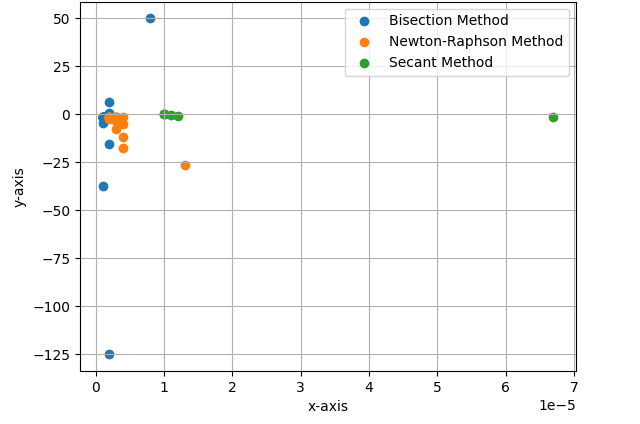
\includegraphics[scale=0.2]{Figure_10.png}
		}
	\end{center}
	\caption{Temperature (T) v/s Entropy (S) diagram for afterburner off, 65 \% nozzle area}
\end{figure}
\subsection{Case- 4:}
For afterburner on, 65 \% nozzle area, the real readings are as follows:
\begin{itemize}
\item Diffuser: $P_1$ = 1.022 bar, $T_1$ = 300 K.
\item Compressor: $P_2$ = 1.845 bar, $T_2$ = 371 K.
\item Turbine: $P_3$ = 1.675 bar, $T_3$ = 820 K.
\item Afterburner: $P_5$ = 1.047 bar, $T_5$ = 1050 K.
\item Nozzle: $P_4$ = 0.935 bar, $T_4$ = 751 K.
\end{itemize}
\clearpage
\begin{figure}[!ht]
	\begin{center}
	   \framebox{
			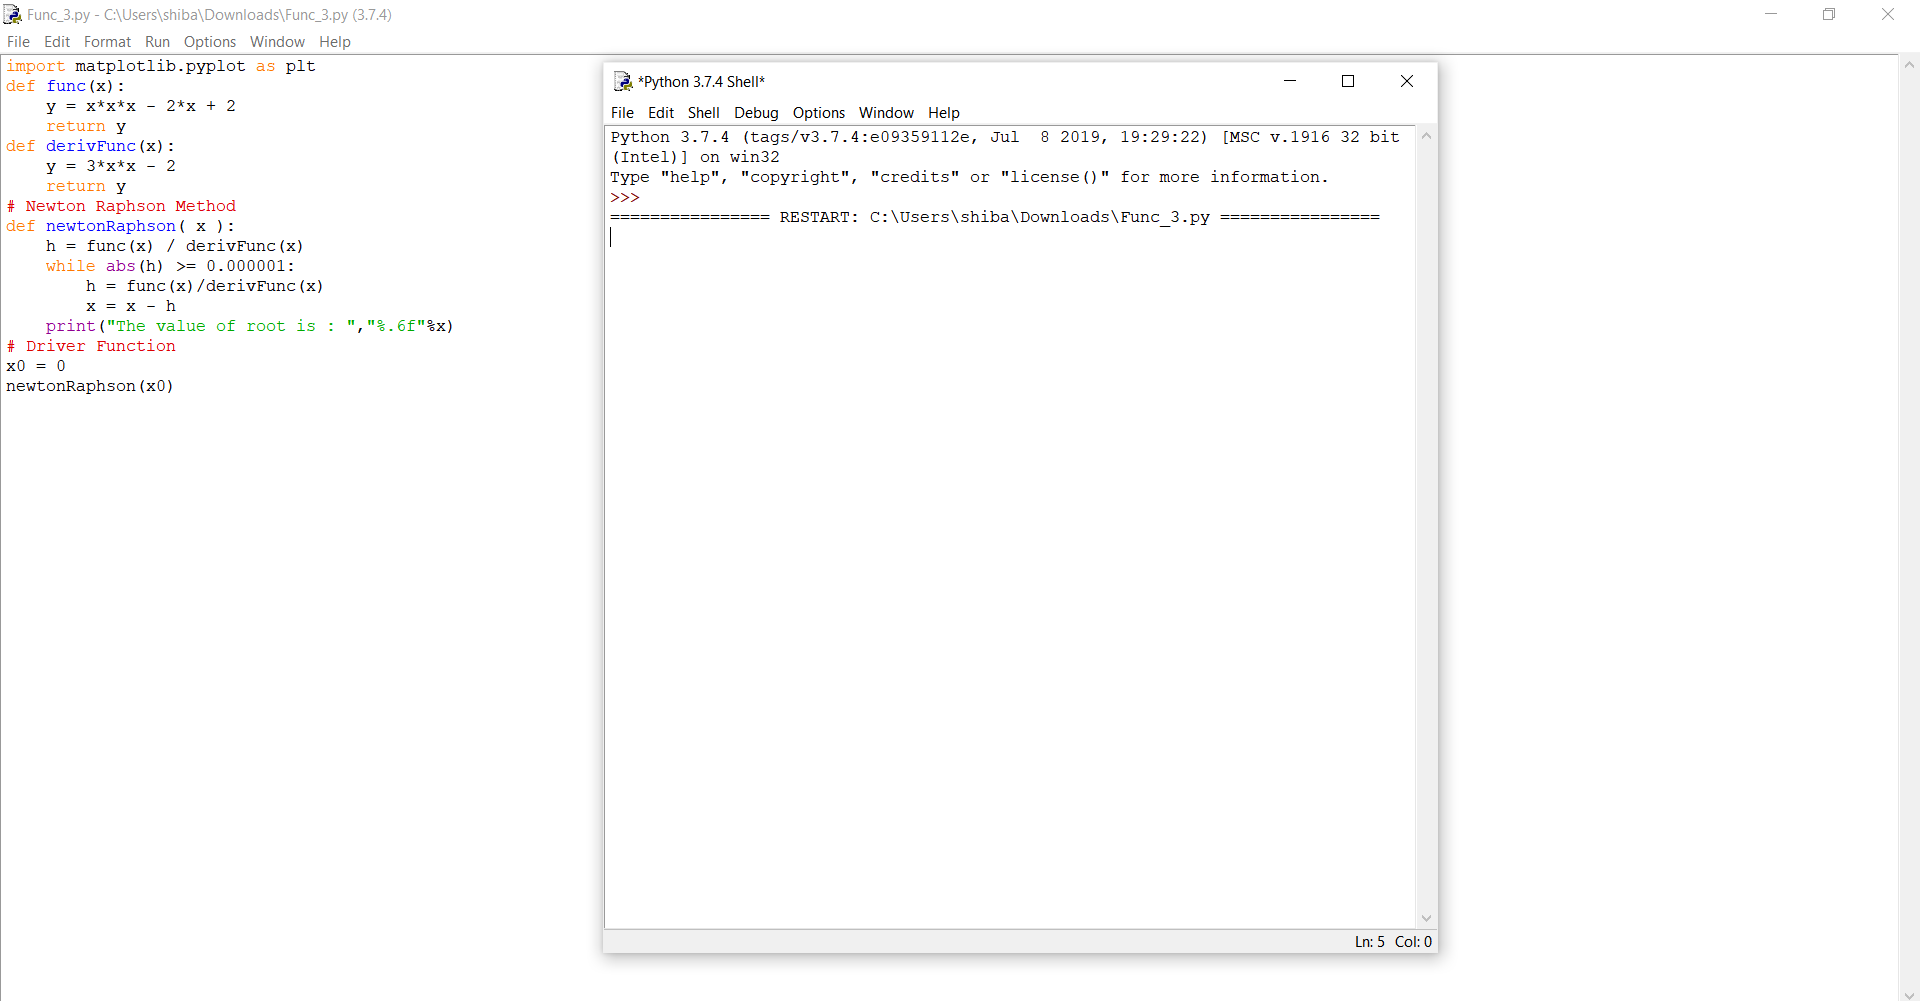
\includegraphics[scale=0.2]{Figure_11.png}
		}
	\end{center}
	\caption{Temperature (T) v/s Entropy (S) diagram for afterburner on, 65 \% nozzle area}
\end{figure}
\section{Observation:}
\begin{itemize}
\item The isoentropic processes shown in the ideal Temperature (T) v/s Entropy (S) cycle are not isoentropic in the real cycle. Thus isoentropic processes are theoretically possible in Turbo-Jet engine but do not take place practically.
\item The Temperature (T) v/s Entropy (S) cycles with 65\% nozzle area reach larger maximum temperature when compared to those with 100\% nozzle area.
\item Real Temperature (T) v/s Entropy (S) cycles have larger maximum entropy compared to those of ideal Temperature (T) v/s Entropy (S) cycles.
\item When the afterburner is used, the maximum entropy and temperature of the air is significantly increased when compared to situation when afterburner is not used. Thus on usage of afterburner significantly higher energy gas is released from the nozzle resulting is similar increase in thrust.
\item The real Temperature (T) v/s Entropy (S) cycle shows increase in entropy in each of the processes. This is inline with the Second Law of Thermodynamics for practical purposes.
\end{itemize}
\section{Conclusion:}
\begin{itemize}
\item The isoentropic processes shown in the ideal Brayton Cycle are not isoentropic in the real Brayton Cycle. Thus isoentropic processes are theoretically possible in Turbo-Jet engine but do not take place practically.
\item From this experiment, we conclude that the Brayton Cycle is very good model to explain the processes happening in a Turbo-Jet engine.
\item The area of the nozzle of the Turbo-Jet engine affects the temperature of the exhaust gases and as a result affecting the thrust of the engine.
\item The afterburner significantly increases the temperature and pressure of the exhaust gas giving a boost to the engine by increasing the thrust momentarily.
\end{itemize}
\end{document}
